\newcommand{\Om}[1][]{\Omega_{\mathrm{#1}}}

\chapter{近独立粒子系统的统计分布}

统计物理是将宏观性质看作是对应微观量的统计平均的微观理论。单粒子的力学规律是决定论的,如量子力学的Schrödinger方程、经典力学中的正则方程或Newton II;而宏观系统的统计规律是非决定论的,用宏观量指定的宏观状态对应大量不同的微观状态。

% 概率基本知识:概念、互斥事件几率的加法定理、独立事件几率的乘法定理、条件概率、二项分布、Poisson分布、Gauss分布、多个随机变量的联合概率分布、统计平均值和涨落等。

\begin{theorem}
	{Schrödinger方程}{Schrödinger equation}
	微观粒子遵从量子力学规律。
	对于单粒子状态,可以通过Schrödinger方程描述:
	\begin{equation}
		\hat H\ket n=\varepsilon_n\ket n,
	\end{equation}
	解得能量本征值$\varepsilon_n$和对应的$\omega_n$个本征量子态$\ket n_1,\ldots,\ket n_{\omega_n}$。

	一个本征值对应多个量子态的情况称为简并(degeneracy),
	$\omega_n$称为简并度。
\end{theorem}

% \begin{example}{一维无穷深势阱}{1-D Infinte Square Potential Well}
% 	一维无穷深势阱能量本征值和简并度
% 	\[
% 		\varepsilon_n=\frac{n^2h^2}{8mL^2},\quad\omega_n=1\quad n=1,2,\ldots.
% 	\]
% 	能级间能量差$\ll$室温下热运动能量(典型值$\SI{25}{meV}$),
% 	因此能量准连续。
% \end{example}

\begin{definition}
	{微观状态和宏观状态}{microstate and macrostate}
	对于多粒子系统,其微观状态(microstate)是粒子按量子态$\ket i_j$的一个分配方式。
	而宏观状态(macrostate)是粒子按能量$\varepsilon_i$的一个分布(distribution)。

	记分布$\{a_i\}$表示有$a_i$个粒子处于能级$\varepsilon_i$,其对应的微观状态数为$\Omega$。
\end{definition}

\begin{corollary}
	由于简并,一个能级$\varepsilon_i$可能有多个量子态$\ket i_j$,因此一个宏观状态可以对应大量不同的微观状态。
\end{corollary}

对于粒子总数$N$、内能$U$和体积$V$确定的平衡态孤立粒子系统,做出两点假设。

\begin{postulate}
	{等概率假设}{equal-probability hypothesis}
	系统的各个微观状态出现的概率相等,即所有分布的总微观状态数$\textstyle\sum_k\Omega_k$的倒数。
\end{postulate}

\begin{remark}
	尽管我们无法直接证明这个假设,但也无从相信某种微观状态更独特,也就是说,我们选取了最简单的均匀分布作为微观状态的先验分布。
\end{remark}

\begin{postulate}
	{最概然分布}{most probable distribution}
	将概率最大的分布作为平衡态分布,称为最概然分布(most probable distribution)。
\end{postulate}

\begin{corollary}
	基于等概率假设,微观状态数$\Omega$最大的分布即为最概然分布。
\end{corollary}

% \begin{remark}
% 	对于宏观系统,粒子数$N$通常在$10^{23}$量级,在这一量级下,最概然分布与实际分布的相对误差极小。
% \end{remark}

\begin{example}
	{}{}
	考虑两个盒子,每个小球有$1/2\vs1/2$的概率在左边或右边的盒子中。
	我们统计左边盒子中的小球数量$X$作为宏观状态分布。
	给定$N$个小球,则$X=k$的分布对应的微观状态数为
	\[
		\Omega(X=k)=\binom Nk:=\frac{N!}{k!(N-k)!}.
	\]
	根据等概率假设,$X$服从二项分布,每种分布的概率为
	\[
		\Pr(X=k)=\frac{\Omega(X=k)}{\sum_{k=0}^N\Omega(X=k)}=\frac1{2^N}\binom Nk.
	\]
	随着$N$的增大,左边盒子中小球数量占比$x:=X/N$的概率密度$f(x)$越来越接近其最概然分布$1/2$,可以证明半高宽$\propto1/\sqrt N$。
	对于宏观系统,粒子数$N$通常在$\NA\sim10^{23}$量级,在这一量级下,实际分布几乎一定是最概然分布。
	\begin{center}
		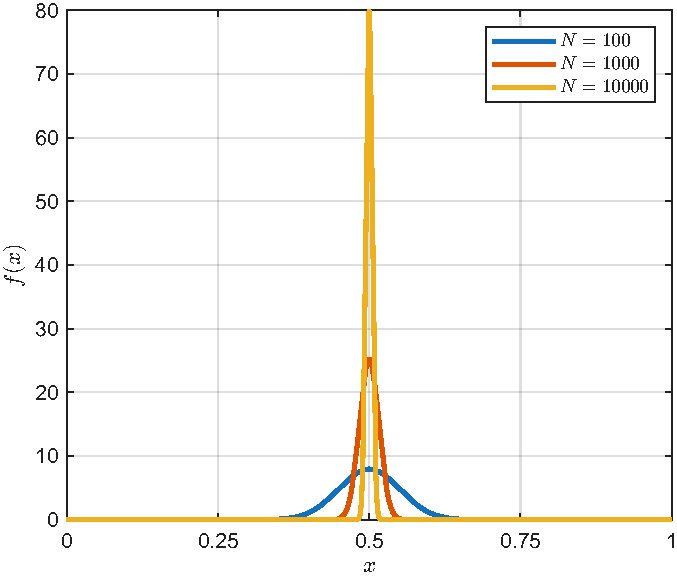
\includegraphics[width=0.6\linewidth]{figures/ML_distribution.pdf}
		\captionof{figure}{分布的概率密度随$N$的变化}
		\label{fig:ML example}
	\end{center}
\end{example}

\section{近独立粒子系统}

\begin{definition}
	{近独立粒子}{nearly independent particle}
	在平均意义下,若
	\begin{center}
		$0<$粒子间作用能$\ll$单个粒子能量
	\end{center}
	则称粒子是近独立的(nearly independent)。
\end{definition}

\begin{corollary}
	对于近独立粒子,整个系统的能量可看成单个粒子能量之和,即\eqref{eq:U=sum a epsilon}。
\end{corollary}

\begin{remark}
	近独立粒子间仍有相互作用,否则无法达到热力学平衡状态。
\end{remark}

\paragraph{经典分布}

下面首先介绍基于经典力学的经典统计力学中的分布——经典Boltzmann分布。
粒子是可以分辨的,比如一些定域分子(如固体晶格).

\begin{definition}{经典Boltzmann系统}{Boltzmann system}
	性质:粒子可以分辨,量子态容纳粒子数不受限制。

	微观状态数:$N$个粒子全排,除去各能级内$a_i$全排,且能级内可占据$\omega_i$中任一态
	\begin{subequations}
		\label{eq:Boltzmann system}
		\begin{equation}
			\Om[M]=N!\prod_i\frac{\omega_i^{a_i}}{a_i!}.
		\end{equation}
	\end{subequations}
	其最概然分布称为(经典) Maxwell-Boltzmann分布,满足
	\begin{equation}
		\label{eq:Boltzmann distribution}
		a_i=\omega_i\e{-\alpha-\beta\varepsilon_i}.
		\tag{\ref{eq:Boltzmann system}b}
	\end{equation}
\end{definition}

\begin{proof}
	假设$a_i,\omega_i\gg 1$,
	由Stirling公式,当$x\gg 1$时,
	\begin{equation}
		% \ln x!=x\ln x-x+\frac12\ln x+\frac12\ln(2\pi )+\bigo\biggkh{\frac1x}.
		\ln x!=x\ln x-x+\bigo(\ln x).
	\end{equation}
	可得
	\[
		\ln\Om[M]\simeq N\ln N+\sum_i a_i\ln\biggkh{\frac{\omega_i}{a_i}}.
	\]
	结合粒子数和内能的条件:
	\begin{subequations}
		\begin{align}
			N&=\sum_i a_i,\\
			\label{eq:U=sum a epsilon}
			U&=\sum_i a_i\varepsilon_i.
		\end{align}
	\end{subequations}
	利用Lagrange乘数法,定义
	\[
		L:=\ln\Om[M]+\alpha\Bigkh{N-\sum_i a_i}+\beta\Bigkh{U-\sum_i a_i\varepsilon_i}.
	\]
	由最概然分布假设,要求
	\[
		\pv L{a_i}=\ln\biggkh{\frac{\omega_i}{a_i}}-\alpha-\beta\varepsilon_i=0
		\implies
		a_i=\omega_i\e{-\alpha-\beta\varepsilon_i}.
	\]
	验证$\p^2L/\p a_i^2=-1/a_i<0$确为极大值点。
\end{proof}

\paragraph{量子分布}

量子粒子与经典粒子是显著不同的,有全同性和自旋两个特点。

\begin{theorem}
	{量子粒子全同性原理}{}
	量子粒子是全同的、不可分辨的,任意交换两个粒子的位置不会改变系统的微观状态。
\end{theorem}

\begin{definition}
	{Bose子和Fermi子}{Boson and Fermion}
	自旋量子数为整数的粒子称为Bose子(Boson),半整数的称为Fermi子(Fermion)。
\end{definition}

\begin{theorem}
	{Pauli不相容原理}{Pauli exclusion principle}
	两个Fermi子不可能处于同一量子态。
\end{theorem}

\begin{definition}{Bose系统}{Bose system}
	性质:粒子不可分辨,量子态容纳粒子数不受限制。

	微观状态数:相当于在$a_i+\omega_i$个粒子$+$空位的间隔中插$a_i$个隔板
	\begin{subequations}
		\label{eq:Bose system}
		\begin{equation}
			\Om[B]=\prod_i\binom{a_i+\omega_i-1}{a_i}=\prod_i\frac{(a_i+\omega_i-1)!}{a_i!(\omega_i-1)!}.
		\end{equation}
	\end{subequations}
	最概然分布称为Bose-Einstein分布,满足
	\begin{equation}
		\label{eq:Bose distribution}
		a_i=\frac{\omega_i}{\e{\alpha+\beta\varepsilon_i}-1}.
		\tag{\ref{eq:Bose system}b}
	\end{equation}
\end{definition}

\begin{proof}
	假设$a_i,\omega_i\gg 1$,
	可得
	\[
		\ln\Om[B]\simeq\sum_i\biggfkh{a_i\ln\biggkh{1+\frac{\omega_i}{a_i}}+\omega_i\ln\biggkh{1+\frac{a_i}{\omega_i}}}.
	\]
	在最概然分布下,
	\[
		\pv L{a_i}=\ln\biggkh{1+\frac{\omega_i}{a_i}}-\alpha-\beta\varepsilon_i=0
		\implies
		a_i=\frac{\omega_i}{\e{\alpha+\beta\varepsilon_i}-1}.
	\]
	验证$\p^2L/\p a_i^2=-\omega_i/a_i(a_i+\omega_i)<0$确为极大值点。
\end{proof}

\begin{definition}{Fermi系统}{Fermi System}
	特点:粒子不可分辨,量子态容纳最多一个粒子。

	微观状态数:从每个量子态的$\omega_i$个空位中挑出$a_i$个粒子
	\begin{subequations}
		\label{eq:Fermi system}
		\begin{equation}
			\Om[F]=\prod_i\binom{\omega_i}{a_i}=\prod_i\frac{\omega_i!}{a_i!(\omega_i-a_i)!}.
		\end{equation}
	\end{subequations}
	最概然分布称为Fermi-Dirac分布,满足
	\begin{equation}
		\label{eq:Fermi distribution}
		a_i=\frac{\omega_i}{\e{\alpha+\beta\varepsilon_i}+1}.
		\tag{\ref{eq:Fermi system}b}
	\end{equation}
\end{definition}

\begin{proof}
	假设$\omega_i\gg a_i\gg 1$,
	可得
	\[
		\ln\Om[F]\simeq\sum_i\biggfkh{a_i\ln\biggkh{\frac{\omega_i}{a_i}-1}-\omega_i\ln\biggkh{1-\frac{a_i}{\omega_i}}}.
	\]
	在最概然分布下,
	\[
		\pv L{a_i}=\ln\biggkh{\frac{\omega_i}{a_i}-1}-\alpha-\beta\varepsilon_i=0
		\implies
		a_i=\frac{\omega_i}{\e{\alpha+\beta\varepsilon_i}+1}.
	\]
	验证$\p^2L/\p a_i^2=-\omega_i/a_i(\omega_i-a_i)<0$确为极大值点。
\end{proof}

\begin{definition}
	{半经典Boltzmann分布}{semi-classical distribution}

	当$\e\alpha\gg 1$时,Bose分布和Fermi分布变为半经典的(semi-classical) Boltzmann分布
	\begin{subequations}
		\begin{gather}
			\Om[S]=\prod_i\frac{\omega_i^{a_i}}{a_i!},\\			
			a_i=\omega_i\e{-\alpha-\beta\varepsilon_i}.
		\end{gather}
	\end{subequations}
	极限条件$\e\alpha\gg 1$称为经典极限条件(classical limit condition),其等价条件为$a_i\ll\omega_i$,因此也可以称为非简并条件(non-degenerate condition)。
\end{definition}

% \begin{proof}
% 	\[
% 		\ln\Om[S]=\sum_i a_i\ln\omega_i-\ln a_i!
% 		=N+\sum_i a_i\ln\biggkh{\frac{\omega_i}{a_i}}.
% 	\]
% \end{proof}

\begin{remark}
	由于粒子不可分辨,半经典与经典Boltzmann分布的微观状态数相差$N!$倍,但二者的最概然分布是一样的。
\end{remark}

\begin{center}
	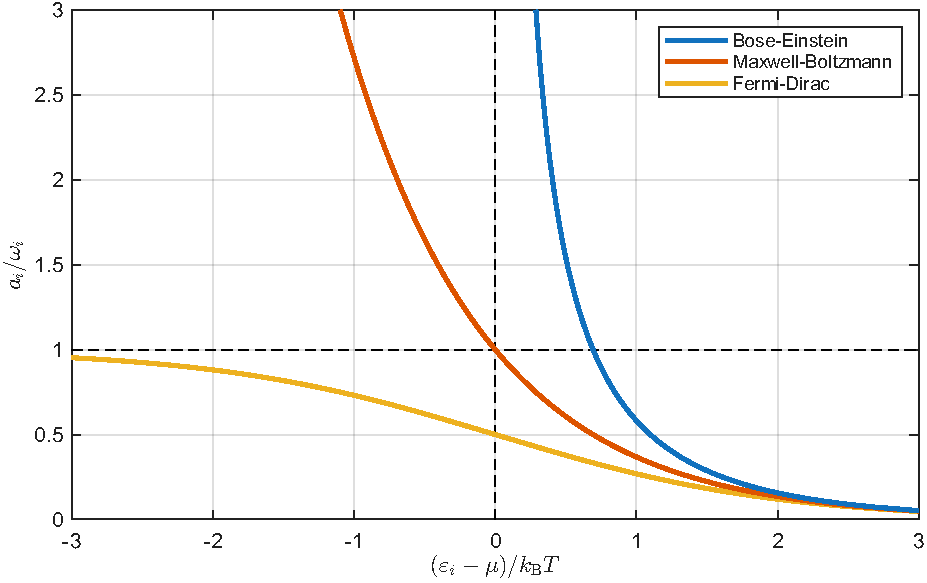
\includegraphics[width=0.8\linewidth]{figures/Boltzmann_Bose_Fermi.pdf}
	\captionof{figure}{三种分布的比较}
	\label{fig:Boltzmann Bose Fermi}
\end{center}

\paragraph{最概然方法误差估计}

\let\oldm\m
\renewcommand{\m}{\mathrm{m}}

在最概然分布$\{a_{i,\m}\}$附近$a_i=a_{i,\m}+\vd a_i$对$\ln\Omega$展开,得
\begin{align*}
	\ln\Omega\{a_i\}&=\ln\Omega\{a_{i,\m}\}+\sum_i\pp{a_i}\ln\Omega\{a_{i,\m}\}\vd a_i+\frac12\sum_i\frac{\p^2}{\p a_i^2}\ln\Omega\{a_{i,\m}\}\vd a_i^2+\bigo(\vd a_i^3)\\
	&\simeq\ln\Omega\{a_{i,\m}\}+0-\frac12\sum_i\frac{\vd a_i^2}{a_{i,\m}}+\bigo(\vd a_i^3).
\end{align*}
对于宏观系统,$N=\textstyle\sum_ia_i\sim 10^{23}$,因此即使分布的相对偏差$\vd a_i/a_{i,\m}\sim 10^{-4}$很小,微观状态数的相对偏差也会大得离谱:
\[
	\frac{\Omega\{a_i\}}{\Omega\{a_{i,\m}\}}\simeq\exp\biggkh{-\frac12\sum_ia_{i,\m}\cdot\frac{\vd a_i^2}{a_{i,\m}^2}}\sim\e{-10^{23-8}}\lll 1.
\]

\let\m\oldm

\section{宏观量的统计表达式}

\begin{definition}{配分函数}{partition function}
	对于(半)经典Boltzmann分布,定义配分函数(partition function)
	\begin{equation}
		Z:=\sum_i\omega_i\e{-\beta\varepsilon_i}.
	\end{equation}
	% 单粒子能级$\varepsilon_i$是外参量$y$的函数。
\end{definition}

\begin{corollary}
	配分函数给出了(半)经典Boltzmann分布的所有信息:
	\begin{subequations}
		\begin{align}
			N&=\e{-\alpha}Z,\\
			% \alpha&=\ln\frac ZN,\\
			\label{eq:U=-NplnZ}
			U&=-N\pv{\ln Z}\beta,\\
			\label{eq:Y=-NplnZ/beta}
			Y_k&=-\frac N\beta\pv{\ln Z}{y_k}.
		\end{align}
	\end{subequations}
\end{corollary}

\begin{proof}
	粒子数
	\[
		N=\sum_i a_i=\sum_i \omega_i\e{-\alpha-\beta\varepsilon_i}=\e{-\alpha}Z
		\implies\e{-\alpha}=\frac NZ.
	\]
	内能
	\[
		U=\sum_i a_i\varepsilon_i=\e{-\alpha}\sum_i \varepsilon_i\e{-\beta\varepsilon_i}=-\frac NZ\pv Z\beta=-N\pv{\ln Z}\beta.
	\]
	内能的微分
	\[
		\d U=\sum_i a_i\d\varepsilon_i+\sum_i \varepsilon_i\d a_i
	\]
	前者是粒子分布不变时能级改变导致的内能变化,对应功$\vd W$;
	后者是能级不变时粒子分布改变导致的内能变化,对应热量$\vd Q$。
	故
	\[
		\sum_k Y_k\d y_k=\vd W=\sum_i a_i\d\varepsilon_i=\sum_i a_i\sum_k\pv{\varepsilon_i}{y_k}\d y_k.
	\]
	可得
	\[
		Y_k=\sum_i a_i\pv{\varepsilon_i}{y_k}=\sum_i \omega_i\e{-\alpha-\beta\varepsilon_i}\pv{\varepsilon_i}{y_k}=-\frac N\beta\pv{\ln Z}{y_k}.
		\qedhere
	\]
\end{proof}

\begin{theorem}{Boltzmann关系}{Boltzmann relation}
	熵与微观态数的关系为
	\begin{equation}
		S=\kB\ln\Omega.
	\end{equation}
	其中$\kB=\SI{1.380649e-23}{\J\per\K}$为Boltzmann常数。
\end{theorem}

\begin{proof}
	考虑
	\begin{align*}
		N\d\ln Z&=N\biggkh{\pv{\ln Z}\beta\d\beta+\sum_k\pv{\ln Z}{y_k}\d y_k}=-U\d\beta-\beta\sum_k Y_k\d y_k\\
		&=-U\d\beta-\beta(\d U-T\d S)=-\d(\beta U)+\beta T\d S.
	\end{align*}
	可得$\d S=\d(N\ln Z+\beta U)/\beta T$,
	两边均为全微分,要求系数$1/\beta T=\kB$为常数,可得
	\begin{align*}
		S&=S_0+\kB(N\ln N+\alpha N+\beta U)
		=S_0+\kB\biggkh{N\ln N+\sum_i a_i(\alpha+\beta\varepsilon_i)}\\
		&=S_0+\kB\biggkh{N\ln N+\sum_i a_i\ln\biggkh{\frac{\omega_i}{a_i}}}
		=S_0+\kB\ln\Om[M].
		\qedhere
	\end{align*}
\end{proof}

\begin{remark}
	对于经典Boltzmann分布,可方便地取$S_0=0$;
	而对于半经典Boltzmann分布,如果要使Boltzmann关系仍成立,应有$S_0=-\kB\ln N!$,或者说 
	\[
		S=\kB\ln\Om[S]=\kB\ln\biggkh{\frac{\Om[M]}{N!}}
		=\kB\biggkh{N+\sum_i a_i\ln\biggkh{\frac{\omega_i}{a_i}}}.
	\]
\end{remark}

% \begin{corollary}
% 	其他宏观量也可以表示,自由能和化学势
% 	\begin{subequations}
% 		\begin{align}
% 			F&=U-TS=-N\kB T(\alpha+\ln N)-TS_0=
% 			\begin{cases}
% 				-N\kB T(\alpha+\ln N),&\text{classical}\\
% 				-N\kB T\alpha,&\text{semi-classical}
% 			\end{cases}
% 			\\
% 			\mu&=\pu[T]FN=-\alpha\kB T.
% 		\end{align}
% 	\end{subequations}
% \end{corollary}

\section{单粒子态的半经典描述}

由理论力学内容,系统的Hamilton量$H\equiv\varepsilon$,广义坐标$q_i$与广义动量$p_i$有关系
\[
	\dot q_i=\pv H{p_i},\quad\dot p_i=-\pv H{q_i}.
\]

\begin{definition}{$\mu$空间}{mu space}
	$\mu$空间是粒子的广义坐标$q_1,\ldots,q_\gamma$与广义动量$p_1,\ldots,p_\gamma$张成的空间。相体积元
	\begin{equation}
		\d\omega=\prod_{i=1}^\gamma\d q_i\nd p_i.
	\end{equation}
	其中$\gamma$为粒子自由度。
\end{definition}

\begin{remark}
	在经典力学中,粒子状态对应$\mu$空间中一个确定的点$(q,p)$;而在(半经典)量子力学中,由Heisenberg不确定性关系$\D q\D p\sim h$,粒子状态(量子态)对应$\mu$空间中的一块相体积。
\end{remark}

\begin{theorem}{极限定理}{limit theorem}
	在大粒子数极限下,一个量子态在$\mu$空间中对应$h^\gamma$的相体积。
\end{theorem}

\begin{corollary}
	由于$(q,p)$是连续的,
	将配分函数写成$\mu$空间中相体积元$\d\omega$的积分形式,
	由极限定理,相体积元$\d\omega$中所含量子态的数量为$\d\omega/h^\gamma$,即
	\[
		Z=\sum_i \omega_i\e{-\beta\varepsilon_i}\to \int_\mu\frac{\nd\omega}{h^\gamma}\e{-\beta\varepsilon}.
	\]
	进一步地,一般情况下系统的能量分布是易求的,我们希望将上式写成能量的积分形式。
	考虑在$(\varepsilon,\varepsilon+\d\varepsilon)$的能量范围内,量子态的数密度(简称态密度)为
	$g(\varepsilon)\d\varepsilon\equiv\d\omega/h^\gamma$,即
	\begin{equation}
		g(\varepsilon)=h^{-\gamma}\dv\omega\varepsilon,
	\end{equation}
	由此可得配分函数$Z$、粒子数$N$和内能$U$的积分表达式
	\begin{subequations}
		\begin{align}
			Z&=\int\zti g(\varepsilon)\e{-\beta\varepsilon}\d\varepsilon,\\
			N&=\e{-\alpha}Z=\int\zti g(\varepsilon)\e{-\alpha-\beta\varepsilon}\d\varepsilon,\\
			U&=-\e{-\alpha}\pv Z\beta=\int\zti g(\varepsilon)\varepsilon\e{-\alpha-\beta\varepsilon}\d\varepsilon.
		\end{align}
	\end{subequations}
\end{corollary}

\subsection*{验证极限定理}

\begin{example}{谐振子}{harmonic oscillator}
	一维谐振子的Hamilton量为
	\[
		\varepsilon=\frac{p^2}{2m}+\frac12m\omega^2x^2.
	\]
	考虑能量$\leq\varepsilon$的相空间体积$\Omega(\varepsilon)$,由椭圆面积公式:
	\begin{equation}
		\Omega(\varepsilon)=\int_{\leq\varepsilon}\d\omega=\pi\sqrt{2m\varepsilon}\sqrt{\frac{2\varepsilon}{m\omega^2}}=\frac{2\pi\varepsilon}\omega
		\implies
		g(\varepsilon)=\frac1h\dv\Omega\varepsilon=\frac{2\pi}{h\omega}.
	\end{equation}
	另一方面,量子力学给出谐振子的能量本征值和简并度为
	\[
		\varepsilon_n=\biggkh{n+\frac12}\hbar\omega,\quad\omega_n=1.
	\]
	$\varepsilon_{n-1}\to\varepsilon_n$只有一个状态,
	相体积为$h$
	\[
		\D\Omega(\varepsilon_n)=\frac{2\pi}\omega\hbar\omega=h.
	\]
	\tcblower
	二维谐振子的Hamilton量为
	\[
		\varepsilon=\frac{p_x^2+p_y^2}{2m}+\frac12m\omega^2(x^2+y^2).
	\]
	由4维单位球体积公式
	\begin{equation}
		\Omega(\varepsilon)=\frac{\pi^2}2\cdot2m\varepsilon\cdot\frac{2\varepsilon}{m\omega^2}=\frac{2\pi^2\varepsilon^2}{\omega^2}
		\implies
		g(\varepsilon)=\frac1{h^2 }\dv\Omega\varepsilon=\frac{4\pi^2\varepsilon}{h^2\omega^2}.
	\end{equation}
	另一方面
	\[
		\varepsilon_n=(n+1)\hbar\omega,\quad\omega_n=n+1.
	\]
	即$\varepsilon_{n-1}\to\varepsilon_n$有$(n+1)$个状态,每个状态的
	相体积为
	\[
		\frac{\D\Omega(\varepsilon_n)}{n+1}=\frac{2\pi^2\hbar^2(2n+1)}{n+1}\to h^2.
	\]
\end{example}
\begin{example}{转子}{rotor}
	转子的Hamilton量为
	\[
		\varepsilon=\frac1{2I}\biggkh{p_\theta^2+\frac1{\sin^2\theta}p_\phi^2}.
	\]
	其中$I$为转动惯量,
	因此
	\begin{gather}\notag
		\Omega(\varepsilon)=\int\d\theta\nd\phi\int\d p_\theta\nd p_\phi=2\pi\int_0^\pi\pi\sqrt{2I\varepsilon}\sqrt{2I\varepsilon\sin^2\theta}\d\theta=8\pi^2I\varepsilon;\\
		\implies
		g(\varepsilon)=\frac1{h^2}\dv\Omega\varepsilon=\frac{8\pi^2I}{h^2}.
	\end{gather}
	另一方面
	\[
		\varepsilon_\ell=\frac{\hbar^2}{2I}\ell(\ell+1),\quad\omega_\ell=2\ell+1.
	\]
	$\varepsilon_{\ell-1}\to\varepsilon_\ell$有$(2\ell+1)$个状态,每个状态的
	相体积为
	\[
		\frac{\D\Omega(\varepsilon_\ell)}{2\ell+1}=\frac{8\pi^2\hbar^2\ell}{2\ell+1}\to h^2.
	\]
\end{example}
\begin{example}{单原子分子}{monatomic molecule}
	在非相对论情形下,单原子分子的Hamilton量为
	\[
		\varepsilon=\frac1{2m}(p_x^2+p_y^2+p_z^2).
	\]
	在体积为$V$的容器中,
	\begin{gather}\notag
		\Omega(\varepsilon)=V\int_0^{\sqrt{2m\varepsilon}}4\pi p^2\d p=\frac{4\pi V}3(2m\varepsilon)^{3/2};\\
		\implies
		g(\varepsilon)=\frac1{h^3}\dv\Omega\varepsilon=\frac{2\pi V}{h^3}(2m)^{3/2}\sqrt\varepsilon.
	\end{gather}
	若考虑自旋,还应乘自旋因子$g_s=2s+1$。

	另一方面
	\[
		\varepsilon_{n_x,n_y,n_z}=\frac{h^2}{8mL^2}(n_x^2+n_y^2+n_z^2),
	\]
	简并度$\omega_{n_x,n_y,n_z}$近似为第一卦限球体积:
	\[
		\omega_{n_x,n_y,n_z}\simeq\frac18\cdot\frac{4\pi}3\biggkh{\frac{8mL^2\varepsilon}{h^2}}^{3/2}=\frac{4\pi}{3}(2\pi\varepsilon)^{3/2}Vh^{-3}.
	\]
	因此每个状态的相体积
	\[
		\frac{\Omega(\varepsilon)}{\omega_{n_x,n_y,n_z}}\simeq h^3.
	\]
	\tcblower
	极端相对论情形下
	\[
		\varepsilon=cp=c\sqrt{p_x^2+p_y^2+p_z^2}.
	\]
	故
	\begin{equation}
		\Omega(\varepsilon)=V\cdot\frac{4\pi}3\biggkh{\frac\varepsilon{c}}^3
		\implies
		g(\varepsilon)=\frac{4\pi V}{h^3c^3}\varepsilon^2.
	\end{equation}
\end{example}
\begin{corollary}
	由\exmref{exm:monatomic molecule} 可知,非相对论情形下
	\[
		\varepsilon=\frac1{2m}\biggkh{\frac h{2L}}^2(n_x^2+n_y^2+n_z^2)=\frac{h^2}{8m}(n_x^2+n_y^2+n_z^2)V^{-2/3}
		\implies
		\pv\varepsilon V=-\frac23\frac\varepsilon V.
	\]
	由\eqref{eq:Y=-NplnZ/beta},可得压强
	\begin{equation}
		p=-\sum_i a_i\pv{\varepsilon_i}V=\frac23\sum_i a_i\frac{\varepsilon_i}V=\frac23\frac UV.
	\end{equation}
	而极端相对论情形下
	\[
		\varepsilon=c\cdot\frac h{2V^{1/3}}\sqrt{n_x^2+n_y^2+n_z^2}
		\implies
		\pv\varepsilon V=-\frac13\frac\varepsilon V.
	\]
	相似的
	\begin{equation}
		p=\frac13\frac UV.
	\end{equation}
\end{corollary}